\section{Self-Attention Defined}
\label{sec:self_attention}
% PROMPT: Show step-by-step derivation of the dot-product attention formula

\begin{figure}[h]
\centering
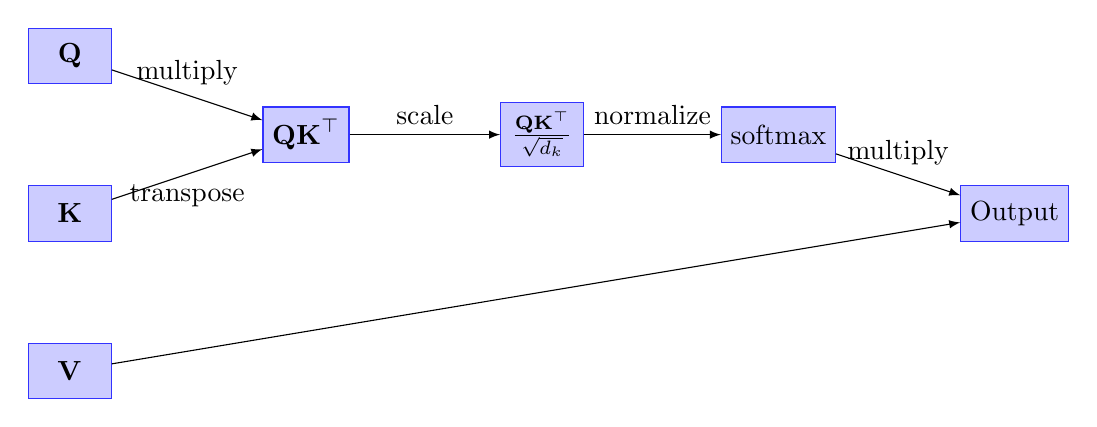
\begin{tikzpicture}[
    node/.style={rectangle, draw=blue!80, fill=blue!20, minimum size=20pt},
    matrix/.style={node, minimum width=30pt},
    vector/.style={node, minimum width=20pt},
    >=latex
]
    % Input matrices
    \node[matrix] (Q) at (0,2) {$\mathbf{Q}$};
    \node[matrix] (K) at (0,0) {$\mathbf{K}$};
    \node[matrix] (V) at (0,-2) {$\mathbf{V}$};
    
    % Matrix multiplication
    \node[matrix] (QK) at (3,1) {$\mathbf{QK}^\top$};
    
    % Scaling
    \node[matrix] (scaled) at (6,1) {$\frac{\mathbf{QK}^\top}{\sqrt{d_k}}$};
    
    % Softmax
    \node[matrix] (softmax) at (9,1) {softmax};
    
    % Final multiplication
    \node[matrix] (output) at (12,0) {Output};
    
    % Arrows and labels
    \draw[->] (Q) -- node[above] {multiply} (QK);
    \draw[->] (K) -- node[below] {transpose} (QK);
    \draw[->] (QK) -- node[above] {scale} (scaled);
    \draw[->] (scaled) -- node[above] {normalize} (softmax);
    \draw[->] (softmax) -- node[above] {multiply} (output);
    \draw[->] (V) -- (output);
\end{tikzpicture}
\caption{Scaled Dot-Product Attention Mechanism: The process transforms query ($\mathbf{Q}$), key ($\mathbf{K}$), and value ($\mathbf{V}$) matrices into attention-weighted outputs through matrix multiplication, scaling, and softmax normalization.}
\label{fig:attention_mechanism}
\end{figure}

\noindent
The \textbf{self-attention} mechanism is a key innovation of the Transformer architecture that allows a model to focus on different parts of a sequence when processing a given token. Unlike recurrent models, which rely on hidden states passed along sequentially, self-attention provides a global view of the entire sequence at each time step.

\subsection{Query, Key, and Value Formulation}
\noindent
In self-attention, each token in a sequence is first mapped to three different vectors:
\begin{itemize}
    \item A \textbf{Query} vector $\mathbf{q}_i$ - represents what the current token is "looking for"
    \item A \textbf{Key} vector $\mathbf{k}_i$ - represents what the token can "match against"
    \item A \textbf{Value} vector $\mathbf{v}_i$ - represents the actual content to be aggregated
\end{itemize}
These vectors are obtained through learned linear transformations of the input embeddings:
\begin{align*}
    \mathbf{Q} &= \mathbf{X}\mathbf{W}^Q \\
    \mathbf{K} &= \mathbf{X}\mathbf{W}^K \\
    \mathbf{V} &= \mathbf{X}\mathbf{W}^V
\end{align*}
where $\mathbf{X}$ is the input sequence and $\mathbf{W}^Q, \mathbf{W}^K, \mathbf{W}^V$ are learnable parameter matrices.

\subsection{Scaled Dot-Product Attention}
\noindent
The attention mechanism computes a weighted sum of values, where the weights are determined by the compatibility between queries and keys. The complete formula is:
\[
\text{Attention}(\mathbf{Q}, \mathbf{K}, \mathbf{V}) 
= \text{softmax}\!\Bigl(\frac{\mathbf{Q} \mathbf{K}^\top}{\sqrt{d_k}}\Bigr) \mathbf{V}
\]

The computation proceeds in four steps (as illustrated in Figure \ref{fig:attention_mechanism}):
\begin{enumerate}
    \item \textbf{Compatibility Scores:} Compute $\mathbf{Q}\mathbf{K}^\top$ to get raw attention scores
    \item \textbf{Scaling:} Divide by $\sqrt{d_k}$ to prevent extremely large values in high dimensions
    \item \textbf{Softmax:} Apply softmax to get a probability distribution over all positions
    \item \textbf{Value Aggregation:} Multiply with $\mathbf{V}$ to get the final attention-weighted output
\end{enumerate}

\subsection{The Importance of Scaling}
\noindent
The scaling factor $\sqrt{d_k}$ is crucial for stable training because:
\begin{itemize}
    \item As dimension $d_k$ increases, dot products grow larger in magnitude
    \item Large values lead to extremely small gradients in the softmax
    \item Scaling keeps the values in a reasonable range where gradients flow well
\end{itemize}

This is related to the concept of softmax temperature $\tau$, where:
\[
\text{softmax}\bigl(\frac{\mathbf{Q}\mathbf{K}^\top}{\sqrt{d_k} \,\tau}\bigr)
\]
controls how "sharp" or "soft" the attention distribution becomes.

\subsection{Masked Self-Attention}
\noindent
For autoregressive tasks like language modeling, we need to ensure that predictions for position $i$ can only depend on positions $\leq i$. This is achieved through masked self-attention:
\[
\text{Attention}(\mathbf{Q}, \mathbf{K}, \mathbf{V}, \mathbf{M}) 
= \text{softmax}\!\Bigl(\frac{\mathbf{Q} \mathbf{K}^\top + \mathbf{M}}{\sqrt{d_k}}\Bigr) \mathbf{V}
\]
where $\mathbf{M}$ is a mask matrix with elements:
\[
M_{ij} = \begin{cases}
    0 & \text{if position } j \leq i \\
    -\infty & \text{otherwise}
\end{cases}
\]

\subsection{Computational Complexity}
\noindent
The self-attention mechanism has complexity characteristics that are important to consider:
\begin{itemize}
    \item Time Complexity: $O(n^2d_k)$ for sequence length $n$
    \item Memory Complexity: $O(n^2)$ for storing attention weights
    \item Parallelization: Highly parallelizable across all positions
\end{itemize}

This quadratic complexity in sequence length has led to various efficient attention variants for handling long sequences, but the basic mechanism remains central to modern LLMs.

% Attention mechanism formula
\begin{equation}\label{eq:attention_mechanism}
\text{Attention}(\mathbf{Q}, \mathbf{K}, \mathbf{V}) = \text{softmax}\!\Bigl(\frac{\mathbf{Q}\mathbf{K}^\top}{\sqrt{d_k}}\Bigr)\mathbf{V}
\end{equation}

% Masked attention
\begin{equation}\label{eq:masked_attention}
\text{Attention}(\mathbf{Q}, \mathbf{K}, \mathbf{V}, \mathbf{M}) 
= \text{softmax}\!\Bigl(\frac{\mathbf{Q} \mathbf{K}^\top + \mathbf{M}}{\sqrt{d_k}}\Bigr) \mathbf{V}
\end{equation}

% Mask matrix definition
\begin{equation}\label{eq:mask_matrix}
M_{ij} = \begin{cases}
    0 & \text{if position } j \leq i \\
    -\infty & \text{otherwise}
\end{cases}
\end{equation}
